\chapterimage{/9/head.jpg} % Chapter heading image
\chapter{Evoluzione non Lineare}\label{9:ch}
Le osservazioni attuali degli ammassi di galassie suggeriscono valori di $\delta \gg 1$, dell'ordine di $100$ o addirittura $1000$. In questi regimi l'approssimazione lineare non è più valida ed è necessario sviluppare una teoria non lineare adeguata. Seppur in qualche caso si riescano a fare i conti con carta e penna (\textit{regime weakly non-linear}, per studiare meglio l'avvicinamento a $\delta = 1$), il più delle volte sono necessarie simulazioni numeriche. 


\section{Approssimazione di Zeldovich}
Questo approccio per descrivere l'evoluzione non lineare delle perturbazioni prevede una distribuzione iniziale omogenea di materia non collisionale, descritta inizialmente da una lagrangiana imperturbata:
\begin{equation}
    \vec{r}(\vec{q},t)=a(t)\vec{q}+\vec{F}(\vec{q},t) \qquad \rightarrow \qquad \vec{r}(\vec{q},t)=a(t)\left[\vec{q}+\delta_+ (t) \vec{G}(\vec{q})\right]\label{eq9:zelapprox}
\end{equation}
dove $\vec{r}=a(t)\vec{x}$ ($\vec{x}$ coordinata comovente), $\vec{F}(\vec{q},t)$ è il termine di displacement, dipendente solo dalla posizione iniziale (sarà il limite di questo metodo) e si è assunta la separabilità: $\vec{F}(\vec{q},t)=a(t)\delta_+ (t)$ per analogia con la teoria lineare. Inoltre il termine di velocità, che quantifica lo spostamento di una particella rispetto alla posizione iniziale, è legato al potenziale gravitazionale iniziale dalla relazione: $\vec{G}(\vec{q})= -\nabla_q \Phi_0 (\vec{q})$. Inoltre si ha:
\begin{equation*}\left.
    \def\arraystretch{1.8}
        \begin{array}{l}
        \vec{v}=\frac{\d{\vec{r}}}{\d{t}}-H\vec{r}=a\frac{\d{\vec{x}}}{\d{t}}=a\;\dot{\delta}_+\nabla_q \Phi_0 (\vec{q}) \\
        \nabla^2_q \Phi_0 = \delta / \delta_+ (t) \quad\rightarrow\quad \delta = \delta_+ (t)\nabla^2_q \Phi_0  \quad (Eq.\; Poisson)
        
    \end{array}\right. 
\end{equation*}

Nell'approssimazione di Zeldovich pertanto, l'approssimazione lineare è svolta sullo spostamento delle particelle, piuttosto che sulla densità. Viene detta teoria di perturbazione \textit{lagrangiana} al primo ordine (precedentemente si è trattata la teoria di perturbazione \textit{euleriana} al primo ordine). Richiede il calcolo del potenziale soltanto all'istante iniziale e prevede che le particelle si muovano su traiettorie rette. Il modello non è più esatto quando due particelle (assunte non collisionali) si incrociano (shell crossing): si viene a creare una singolatità. L'equazione (\ref{eq9:zelapprox}) mappa univocamente le coordinate $\vec{q}$ e $\vec{r}$, quindi fintantoché due traiettorie non si incrociano, per piccoli spostamenti si ha:
\begin{equation}
    \rho(\vec{r},t)\d{^3r}=\overbar{\rho} (t_i) \d{^3q} \quad \rightarrow \quad \rho(\vec{r},t) = \frac{\overbar{\rho} (t)}{|J(\vec{r},t)|}
\end{equation}
dove $|J(\vec{r},t)|$ è il determinante della matrice Jacobiana. Dal mometo che il fluido è irrotazionale, la matrice è simmetrica e quindi può essere diagonalizzata:
\begin{equation}
    \rho(\vec{r},t)=\overbar{\rho} (t) \left[\left(1-\delta_+ \lambda_1\right)\left(1-\delta_+ \lambda_2\right)\left(1-\delta_+ \lambda_3\right)\right]^{-1}
\end{equation}
Per tempi sufficientemente piccoli, per cui $\delta_+ (t)\lambda_i\ll 1$, si ha:
\begin{equation}
    \delta\simeq -\left(\lambda_1 + \lambda_2 + \lambda_3\right)\delta_+(t)
\end{equation}
Se i tre autovalori $\lambda_i (\not\propto t)$ sono $<0$ la densità diminuisce, se sono $>0$ la densità cresce, ma può anche verificarsi che diverga all'infinito (\textit{shell crossing}). Nel caso in cui tutti e tre gli autovalori siano uguali si ha espansione/collasso sferico, altrimenti è ellissoidale. Per due negativi e uno positivo collasso planare e per due positivi e uno negativo collasso su un filamento. Questo modello regge bene fino a $\delta\sim 5$, ma può essere sviiluppato a ordini superiori. 
Si può dimostrare che la formazione delle strutture avviene inizialmente su piani (\textit{pancake di Zeldovich}), mentre al passare del tempo sono preferite strutture filamentose che convergono in nodi. 

\section{Collasso sferico}
Si considerano le perturbazioni come universi chiusi immersi in un universo di background EdS e si assume che siano perfettamente sferiche e ferme rispetto al flusso di Hubble $v_{pec}=0$. Nella Sezione \ref{ch6:chilovoleva} era stato ricavato l'andamento delle perturbazioni dopo l'equivalenza che rispetto un generico istante iniziale diventa:
\begin{equation}
    \delta = \delta_+ \left(\frac{t}{t_i}\right)^{2/3} + \delta_- \left(\frac{t}{t_i}\right)^{-1}\label{eq9:delta}
\end{equation}
ora la perturbazione decrescente non viene più trascurata. In regime lineare: $v = ia\dot{\delta}/k_x $, inoltre in un universo EdS: $a\propto t^{2/3}$ (per i tempi in esame). Indicando con il pedice $x$ le coordinate comoventi e con $r$ quelle fisiche ($k_r = k_x /a$) si ha: 
\begin{equation}
    v= \frac{i}{k_x \left(t/t_i\right)^{-2/3}}\;\frac{1}{t_i}\left[ \frac{2}{3}\delta_+ \left(\frac{t}{t_i}\right)^{-1/3} - \delta_- \left(\frac{t}{t_i}\right)^{-4/3}    \right]  
\end{equation}
Applicando l'assunzione $v(t_i)=0$ e l'equazione \ref{eq9:delta} si ha:
$$
\delta_- (t_i)= \frac{2}{3}\delta_+(t_i)\quad \rightarrow \quad \delta (t_i) = \frac{5}{3}\delta_+ (t_i)
$$

Il parametro di densità della perturbazione vale: $\Omega_p(t_i)=\rho_p(t_i) / \rho_{crit} = \Omega (t_i) (1+\delta(t_i))$, dove $\Omega (t_i)$ è il parametro di densità dell'universo di background. La \textbf{condizione per il collasso della perturbazione sferica} è $\Omega_p (t_i)>1$, ossia:
$$
\Omega (t_i) (1+\delta(t_i)) > 1
$$
Se $\Omega (t_i)\geq 1$ tutte le perturbazioni collassano, mentre se $\Omega (t_i)< 1$ si introduce un \textbf{valore di soglia} che deve essere superato affinché si possa avere collasso:
\begin{equation}
    \delta_+ (t_i) > \frac{3}{5}\left(\frac{1-\Omega (t_i)}{\Omega (t_i)}\right)
\end{equation}

La condizione per un universo di background di Friedmann con sola materia diventa:
$$
\delta_+ (t_i) > \frac{3}{5}\frac{1-\Omega_i}{\Omega_i (1+z_i)}
$$

Questo significa che esiste una soglia che va superata in tempo utile (aumenta col tempo) se si vuole avere collasso. Questa è sempre superata in universi chiusi e piatti $\Omega_i \geq 1$, ma non per quelli aperti. L'evoluzione del piccolo universo chiuso con cui è stata approssimata la perturbazione prevede un $t_{max}$ a cui si ha un $a_{max}$, $\dot{a}(t_{max})$ e quindi una successiva contrazione (\textit{big crunch}), inoltre $\rho_p (t_{max})\propto a_{max}^{-3}$. Si può dimostrare che la densità della perturbazione al tempo del massimo vale:
\begin{equation}
    \rho_p (t_{max})=\frac{3\pi }{32\; G} \; \frac{1}{t_{max}^2}
\end{equation}
Confrondola con la densità del background ($\rho(t_{max})=(6\pi \; G \; t_{max}^2)^{-1}$) si ottiene:
$$
\chi (t_{max}):= \frac{\rho_p(t_{max})}{\rho (t_{max})}= \frac{9\pi^2}{16}\approx 5.6 \qquad \rightarrow\qquad \delta^{nLin} (t_{max})= \chi -1 \approx 4.6
$$
ovvero, al momento del \textit{turnaround}, la perturbazione è già altamente non lineare e le assunzioni fatte per questo modello non valgono più. Seguendo puramente la trattazione lineare avremmo ottenuto un valore:
$$
\delta^{lin}(t_{max})=\frac{3}{5} \left(\frac{3\pi}{4}\right)^{2/3}\approx 1.07
$$
Il risultato è sbagliato di un fattore 4 e deve ancora iniziare il collasso vero e proprio.



\section{Fase di virializzazione}
Ci si aspetta che la perturbazione, assunta come universo chuiso, ricollassi su sé stessa in un tempo $t_{coll}=2t_{max}$. Tuttavia le perturbazioni di materia non possono collassare in un punto: entrano in gioco il riscaldamento nel caso di materia barionica e la dispersione di velocità nel caso di materia oscura. La perturbazione si virializza su un dato raggio calcolabile dal teorema del viriale:
\begin{equation*}\left\{
    \def\arraystretch{1.5}
        \begin{array}{ll}
            2T+V=0 \\
            E=T+V
    \end{array}\right. \quad\Leftrightarrow  \quad E(t_{vir})=\frac{V}{2}= -\frac{1}{2}\frac{3}{5}\frac{G M^2}{R_{vir}}\equiv E(t_{max})=-\frac{3}{5}\frac{GM^2}{R_{max}}
\end{equation*}
dove si è posto per conservazione dell'energia, $E(t_{vir})\equiv E(t_{max})$, periodo in cui la velocità e quindi l'energia cintica è nulla. Da questa relazione si ha che la perturbazione si virializza quando: $R_{vir}=R_{max}/2$, ossia quando $\rho_p (t_{vir})=8 \rho_p (t_{max})$. Le simulazioni mostrano che il tempo in cui avviene la virializzazione è $t_{vir}\simeq 3 t_{max}$. Con questi dati si possono stimare due quantità fondamentali:
\begin{equation}\left\{
    \def\arraystretch{1.5}
        \begin{array}{ll}
        \frac{\rho_p (t_{coll})}{\overbar{\rho}(t_{coll})}=8 \frac{\rho_p (t_{max})}{\overbar{\rho}(t_{max})}\left(\frac{t_{coll}}{t_{max}}\right)^2 \simeq 180\\
        \frac{\rho_p (t_{vir})}{\overbar{\rho}(t_{vir})}=8 \frac{\rho_p (t_{max})}{\overbar{\rho}(t_{max})}\left(\frac{t_{vir}}{t_{max}}\right)^2 \simeq 400
    \end{array}\right. 
\end{equation}
dove si è utilizzata la quantità $\chi (t_{max})$ calcolata nella sezione precedente. Questi due valori corrispondono a dei $\delta$ (sottraendo 1) decisamente non lineari. Svolgendo ingenuamente i conti con la teoria puramente lineare, si sarebbe ottenuto:
\begin{equation}\left\{
    \begin{array}{l}
    \delta^{lin}(t_{coll})=\delta^{lin}(t_{max})\left(\frac{t_{coll}}{t_{max}}\right)^{2/3}\simeq 1.68\\
    \delta^{lin}(t_{vir})=\delta^{lin}(t_{max})\left(\frac{t_{vir}}{t_{max}}\right)^{2/3}\simeq 2.2
\end{array}\right. 
\end{equation}

La teoria non lineare predice giustamente numeri molto grandi, simili a quelli osservati nelle strutture formate, quella lineare sbaglia di due ordini di grandezza. I limiti della trattazione non lineare svolta sono: collasso sferico (l'approssimazione di Zeldovich suggerisce che è impossibile che due autovalori siano perfettamente uguali), la dipendenza forte dalla cosmologia (densità media della materia legata a $\Omega_m$, evoluzione con $t^2$ dovuta all'assunzione EdS). In regime lineare i numeri sono compleatamente sballati, ma dipendono molto meno dalla cosmologia (e.g. $1.68\pm 0.05$). In ogni caso gli osservativi utilizzano, a partire dalle regioni più interne: $R_{2500}, R_{500}, R_{200}$.

\begin{figure}[H]
    \centering
    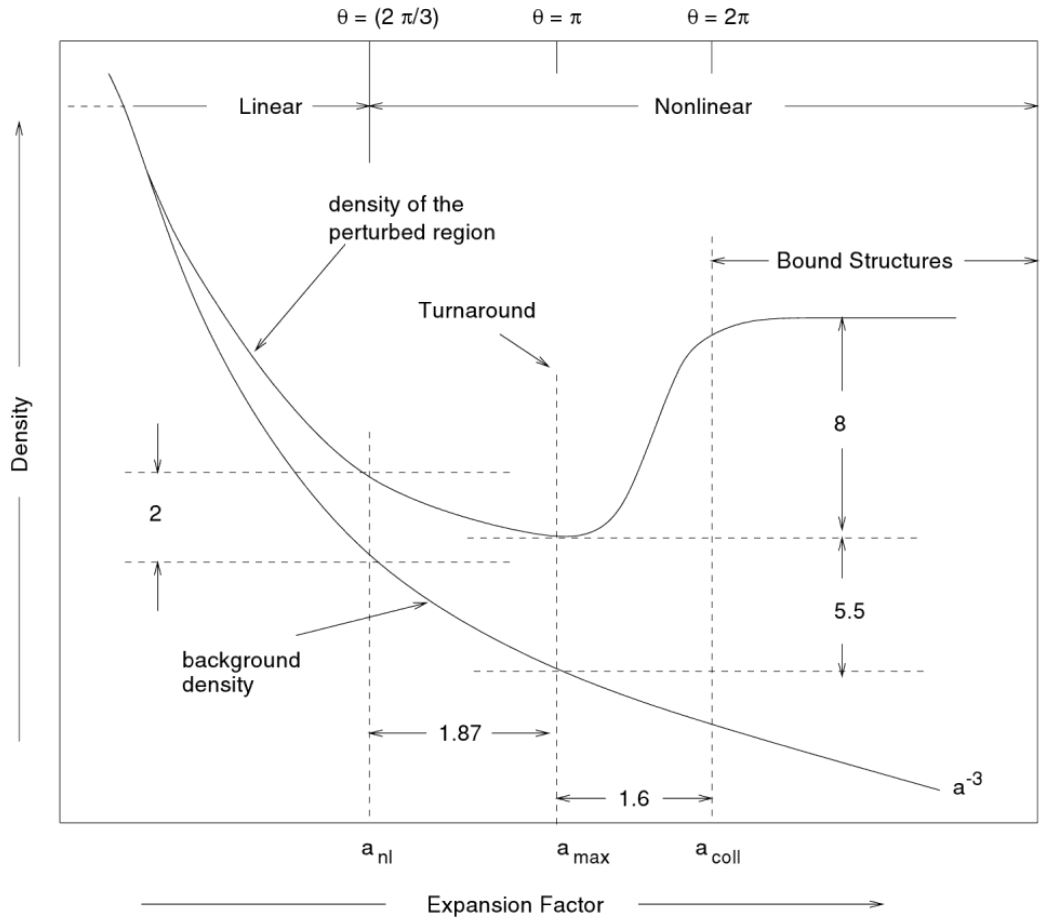
\includegraphics[width=.75 \textwidth]{Pictures/9/Padmanabhan.jpg}
    \caption{Evoluzione di una regione sovredensa in approssimazione sferica \textit{top-hat}. Dopo $a_{coll}$ il contrasto continua a crescere perché diminuisce la densità di background (From: \cite{padmanabhan2002}).}
\end{figure}



\section{Teoria di Press–Schechter}
La funzione di massa rappresenta la densità numerica di oggetti con massa compresa tra $M$ e $M+\d{M}$. Ammettendo che tutti gli oggetti abbiano lo stesso rapporto massa/luminosità (falso), si traduce nella funzione di luminosità: 
\begin{equation}
    \d{N}=n(M)\d{M} = \Phi(L)\d{L} \qquad \rightarrow \qquad \Phi(L)=n(M)\frac{\d{M}}{\d{L}}\simeq n(M)\left\langle \frac{M}{L} \right\rangle 
\end{equation}
Da un punto di vista teorico si studia la funzione di massa e non quella di luminosità perché i barioni fanno brutte cose. Il modello più interessante è la funzione di massa di Press-Schechter, legato alla funzione di luminosità di Schechter. Il campo di densità filtrato su una certa scala $R$ è stato descritto con l'operazione di convoluzione, in particolare: $\delta_M (\vec{x})=\delta(\vec{x}) * W(R)$. La distibuzione delle perturbazioni attuale è rappresentata in Figura (\ref{fig8:ultima}), per conoscere quanti oggetti si sono formati bisognerebbe integrare la curva a partire da $\delta_M = 180$ (assumendo EdS). Sia la non-gaussiana, sia il valore $180$ non sono ricavabili facilmente e hanno forti dipendenza dalle assunzioni, come già discusso. 

I signori Press e Schechter hanno pensato che modellando l'evoluzione in regime lineare (la gaussiana si allarga, ma rimane gaussiana) e utilizzando quindi la soglia calcolata in tale approssimazione ($\delta^{lin}(t_{coll})=1.68$), i due errori si auto-compensano. La massa che finisce negli oggetti che collassano è quindi quella corrispondente alla coda gaussiana superiore alla soglia $1.68$. Le simulazioni confermano la bontà di questa approssimazione.

Dato che l'operazione di filtraggio non altera la gaussianità primordiale si ha:
\begin{equation*}
    P(\delta_M)=\frac{1}{\sqrt{2\pi \sigma_M^2}}e^{-\delta_M / (2\sigma_M^2)}\quad \to \quad P_{>\delta_{coll}}(M)=\int_{1.68}^\infty P(\delta_M)\d{\delta_M}= \frac{1}{2}\left[1-\mathrm{erf}\left(\frac{\delta_{coll}}{\sqrt{2}\sigma_M}\right)\right]
\end{equation*}

La cosmologia entra pochissimo in $\delta_{coll}$, ma pesantemente in $\sigma_M=f(M,z)$. La probabilità che avvenga il collasso anche per un oggettesimo di massa $M= 0$ ($R\to 0$, $\sigma_M \to \infty$, $\mathrm{erf}\to 0$) tende a $1/2$, nonostante per definizione dovrebbe essere $1$ (non si è posto nessun filtro limite). Questo è dovuto al fatto che si sta ignorando il contributo della parte sottodensa, ma anche questa potrebbe contribuire al collasso, pertanto si metterà a mano un fattore $2$ (proprietà di simmetria della gaussiana). Per rifasi alla definizione di funzione di massa si ha l'uguaglianza:
\begin{equation*}
    2\: \left[P_{>\delta_{coll}}(M)-P_{>\delta_{coll}}(M+\d{M})\right]\frac{\overbar{\rho}_m }{M}\d{M}=n(M)\d{M}
\end{equation*}
La quantità fra parentesi quadre è necessariamente positiva perchè filtrando su scale maggiori la probabilità (varianza di massa) diminuisce. Proseguendo con i conti:
\begin{equation*}
    n(M)\d{M}= 2 \overbar{\rho}_m \left\lvert \frac{\d{P_{>\delta_{coll}}}}{\d{\sigma_M}}\right\rvert \left\lvert \frac{\d{\sigma_M}}{\d{M}}\right\rvert \d{M}=2 \overbar{\rho}_m\; \frac{1}{\sqrt{2\pi \sigma_M^2}}\frac{\delta_{coll}}{\sigma_M}e^{-\delta_{coll}/(2\sigma_M^2)}\; \frac{\sigma_M}{M} \left\lvert \frac{\d{\ln \sigma_M}}{\d{\ln M}}\right\rvert \; \d{M}
\end{equation*}
dove si utilizza la derivata rispatto al logaritmo perché la funzione è puù smooth. La \textbf{funzione di Press-Schechter} è quindi:
\begin{equation}
    n(M)\d{M}= \sqrt{\frac{2}{\pi}}  \;\frac{\overbar{\rho}_m\; \delta_{coll}}{\sigma_M\; M^2}\left\lvert \frac{\d{\ln \sigma_M}}{\d{\ln M}}\right\rvert \; \d{M}
\end{equation}

Assumendo uno spettro power-law del tipo: $\sigma_M\propto (M/M_0)^{-\alpha}$ dove $\alpha = (n+3)/6$ e svolgendo la sostituzione: $M_*^2=M_0^2 (2/\delta_{coll})^{1/2\alpha}$, si ha:
\begin{equation}
    n(M)\d{M}= \sqrt{\frac{2}{\pi}} \frac{\overbar{\rho}_m\; \alpha}{M_*^2}\left(\frac{M}{M_*}\right)^{\alpha -2} e^{-(M/M_*)^{2\alpha}}\d{M}
\end{equation}

Si ha un taglio esponenziale che agisce dalla massa $M_*$ preceduto da un andamento a legge di potenza con esponente $\alpha-2$. La stessa situazione si ha per la funzione di luminosità assumendo un rapporto $M/L$ costante al variare della massa. Osservativamente si ha una pendenza $\approx -1$ per le galassie, che si traduce in un $\alpha -2=-1 \to n = 3$. Questo valore non è compatibile con i valori aspettati ($n\approx -2$) per l'indice dello spettro della CDM su scala delle galassie. Ossia, c'è una sovrabbondanza di aloni di materia oscura rispetto alle galassie (non c'è una relazione 1:1) su scale così piccole. Questo è dovuto ai barioni.

\begin{figure}[H]
    \centering
    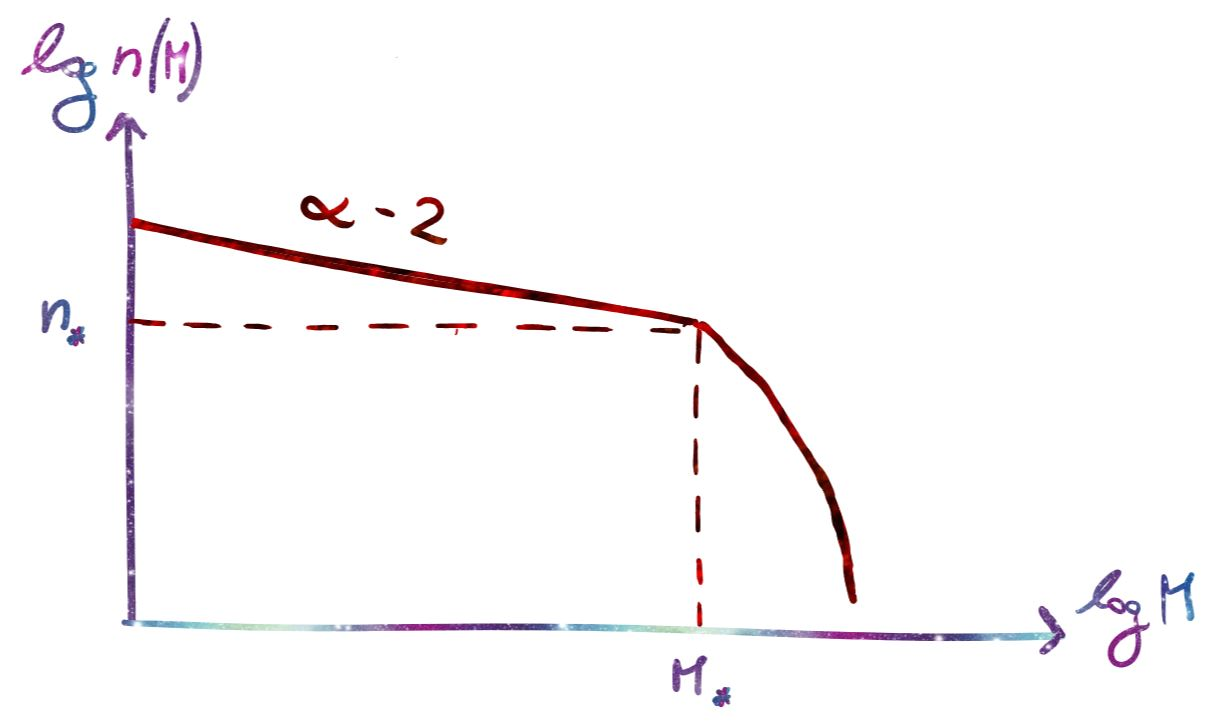
\includegraphics[width=.7 \textwidth]{Pictures/9/ps.jpg}
    \caption{Funzione di Press-Shechter}
\end{figure}

La quantità $M_*$ è legata alla massa tipica degli oggetti che si stanno formando in un dato periodo. Oggi $M_*$ corrisponde a quella degli ammassi di galassie ($10^{15}M_\odot$). Nonostante ne sia previsto un piccolo numero, questi oggetti massicci sono facili da detectare e dipendono poco dalla miscrofisica: studiando la coda della funzione di massa si possono porre ottimi contraints. La funzione di massa può essere tradotta sotto forma di probabilità di trovare oggetti di data temperatura, luminosità X o dispersione di velocità: $T_x\propto \langle v^2\rangle \propto M^{2/3}(1+z)$; $L_x \propto R^3 n^2 T_x^{1/2}\propto M^{4/3}(1+z)^{7/2}\propto T_x^2 (1+z)^{3/2}$ (valide assumendo solo il contributo della gravità).  

In conclusione, la formula è approssimata: si assume collasso sferico (si può correggene analiticamente per il collasso ellisoidale, Sheth \& Tormen), si è inserito in modo arbitrario il fattore 2 (si può verificare con la teoria dei random walk che è corretto). Se ci si fida delle simulazioni N-body (anche lasciando libero $\delta_{coll}$), si hanno forme più complesse (Tinker, Despali...), ma non troppo diverse. La cosmologia si nasconde in $\overbar{\rho}_m$, fortemente sensibile a $\Omega_m$ e in $\sigma_M^2\propto \int k^2 \mathcal{P}(k)W^2(k,R)\d{k}$ sensibile fortemente alla normalizzazione $A$ e leggermente (perché integrate) a $n_s$ e alla funzione di trasferimento $T^2(k)$. Per superare una data soglia $\delta_{coll}$ a un dato tempo $t$ si hanno infinite combinazioni possibili di $A$ e $\Omega_m$, e.g. aumentando $A$ in un universo con $\Omega_m$ minore ($\delta_+ \propto \Omega_m^{0.55}$). Vi è degenerazione tra $\Omega_m$ e $\sigma_8$ (in letteratura si usa questo valore definito in precedenza). 

In particolare gli ammassi sono sensibili a:
\begin{equation}
    S_8 := \sigma_8 \left(\frac{\Omega_m}{0.3}\right)^{0.5}
\end{equation}
che viene quindi misurata contando gli ammassi. Per rompere la degenerazione è necessario contare gli ammassi al variare del redshift e studiare l'evoluzione di $n(M)$. Guardando indietro nel tempo, ci si aspetta più ammassi negli universi a basso $\Omega_m$ rispetto a quelli ad alto $\Omega_m$ (ma sempre meno rispetto al numero attuale). L'unico problema non piccolo è che la massa non è un osservabile diretto.

\begin{figure}[H]
    \centering
    \subfloat[]{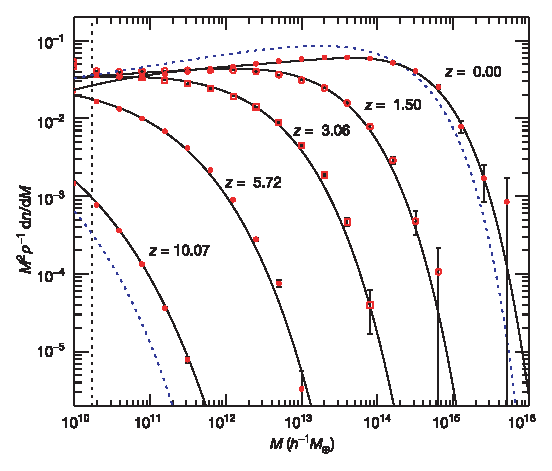
\includegraphics[width=.5\textwidth]{Pictures/9/nmz.eps}}$\;\;$
    \subfloat[]{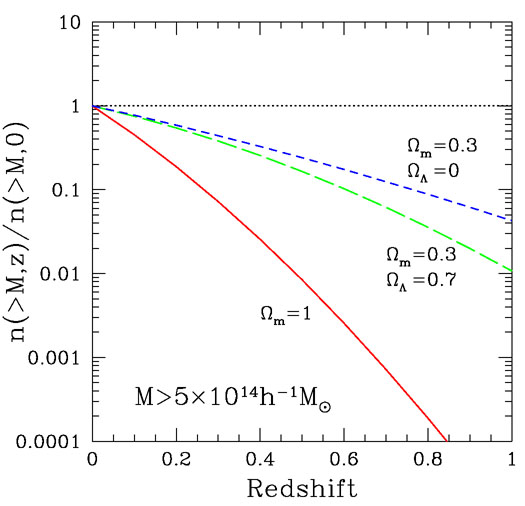
\includegraphics[width=.455\textwidth]{Pictures/9/psevol.jpg}}
    \caption{(a) La funzione $n(M,z)$ da la densità comovente di aloni meno massicci di M. Linea continua: modello Shet-Tormen, linea tratteggiata: modello Press-Shechter, pallini rossi: simulazione Millennium Run. (From: \cite{2005Natur.435..629S}); (b) L'evoluzione di un'altra quantità, $n(>M,z)$ da un'altra prospettiva.}
\end{figure}

\newpage
\section{Simulazioni numeriche}
Le simulazioni numeriche vengono divise in due grandi classi: quelle puramente n-body e quelle idrodinamiche che includono anche effetti barionici su diverse scale (eventualmente shocks, ecc...). Il modello di base di formazione delle strutture si basa sulle instabilità gravitazionali guidate dalla materia oscura. L'universo viene suddiviso in tanti volumetti (particelle) e la sua evoluzione può essere studiata risolvendo il problema degli n-body: essendo $n\gg 3$ si ricorre all'integrazione numerica. 
Il set di equazioni più semplici è: 
\begin{equation}\left\{
    \def\arraystretch{1.5}
        \begin{array}{ll}
        F_i = Gm_i \sum_{i\neq j} m_j/r_{ij}^2 \\
        v_i(t+\Delta t)=v_i (t)+\frac{F_i}{m_i} \Delta t + \mathcal{O} (\Delta t^2) \\
        x_i(t+\Delta t)=x_i (t)+v_i \Delta t + \mathcal{O} (\Delta t^2)
    \end{array}\right. 
\end{equation}

Inizialmente si calcola la forza e il modo in cui viene svolto questo processo definisce diverse categorie di codici n-body:

\begin{example}[Particle-Particle (PP)]
    La forza che agisce sulla $i-esima$ particella viene calcolata in modo naturale sommando i contributi di tutte le altre particelle, una ad una. $$ \vec{F}_i \propto \frac{\vec{x}_i-\vec{x_j}}{|\vec{x}_i-\vec{x_j}|^3}$$È molto semplice costruire il codice, ma è molto costoso dal punto di vista computazionale. Con $N$ particelle le distanze da calcolare diventano $N^2$ ad ogni passo temporale, pertanto diventa anche difficile aumentare la risoluzione della simulazione. Inoltre, se due particelle si avvicinano troppo, la forza diverge all'infinito (non avviene fisicamente ed è brutta numericamente), quindi si introduce un parametro di \textit{softening} della forza. In questo modo si può impedire che due oggetti si avvicinino di più della loro dimensione. 
    \\ ${\color{green} \blacktriangle  } $ Calcolo esatto della forza tra particelle (importante per sistemi collisionali). \\ ${\color{red} \blacktriangledown } $ Complessità $\mathcal{O} (N^2)$, softening necessario per evitare divergenza.
 
\end{example}   


\begin{example}[Particle Mesh (PM)]
 Si trattano come quantità di campo tutte le quantità che possono essere assunte tali. Densità, potenziale gravitazionale e quindi forza vengono calcolate interpolando quantità in griglia. $$ \rho (\vec{x}_{ijk})=\sum_{l=1}^N W(\vec{x}_l - \vec{x}_{ijk}) \; \rho(\vec{x}_l)$$ Cioè la densità in un punto ${ijk}$ della griglia si ottiene pesando i contributi di tutte le altre particelle attraverso il cosiddetto \textit{kernel} $W$ che determina l'interpolazione. Un $W$ gaussiano non andrebbe mai a zero, altri filtri interessanti sono:
 \begin{itemize}
     \item[-] \textbf{Nearest Grid Point} (NGP): ogni particella contribuisce solo al nodo più vicino. La densità diventa discontinua.
     \item[-] \textbf{Cloud In Cell} (CIC): ogni particella contribuisce solo ai 4 nodi più vicini in maniera inversamente proporzionale al quadrato della distanza (2D). La derivata prima è discontinua.
     \item[-] \textbf{Triangular Shaped Cloud} (TSC): ogni particella contribuisce solo ai 8 nodi più vicini in maniera inversamente proporzionale al quadrato della distanza (3D). In questo caso, la funzione è più smooth e la discontinuità si è spostata alla derivata seconda. In genere si utilizza questo.
 \end{itemize}

 Partendo dalle posizioni delle particelle si calcolano le densità per ogni punto griglia utilizzando le interpolazioni precedenti. Utilizzando la griglia regolare, si possono semplificare le equazioni trasformandole nello spazio di Fourier: $\delta\to \delta_k$, in questo modo diventano semplici moltiplicazioni. La forza ottenuta dello spazio di Fourier si antitrasforma per avere la forza nello spazio reale su ogni punto della griglia. La forza che agisce sulla particella $i-esima$ si ottiene interpolando.

[Quindi in questo modo posso fregare la gravità (non locale) e calcolarla utilizzando una quantità locale $\delta_k$... no, bugia! $\delta_k$ ha informazioni su tutte le scale $k$, la gravità non ha cambiato la sua natura, ad oggi... ]
 \\ ${\color{green} \blacktriangle  }$ Complessità $\mathcal{O} (N\log N)$. 
 \\ ${\color{red} \blacktriangledown } $ Risoluzione limitata dalla costruzione della griglia. Migliorabile combinandolo col metodo Particle-Particle, \textbf{codici P3M}: conti diretti per particelle vicine, in griglia per particelle lontane). Migliorabile anche con metodi che rifiniscono la griglia: \textbf{Adaptive Particle Mesh}.

\end{example}  

\begin{example}[Tree code (HT)]
   Sfruttano il concetto di baricentro e la teoria dei grafi. Inizialmente si costruisce un albero gerarchico: ogni regione viene scomposta in sottoregioni fintantoché non contiene al più una particella (Fig. \ref{fig9:treecode}). Se una regione è arbitrariamente molto distante dalla particella $i-esima$ in analisi, viene trattata come un'unica particellona e non vengono considerate le sue sottoregioni. Più ci si avvicina alla particella, più si scompongono i contributi delle sottoregioni (si scende di gerarchia). Eventualmente, nelle zone prospicienti si potrebbe calcolare direttamente la forza tra due particelle come nel metodo PP. Può essere problematico memorizzare tutti i livelli dell'albero gerarchico, ma è più efficiente. Questo metodo ad oggi è quello che va per la maggiore.
   \\ ${\color{green} \blacktriangle  }$ Complessità $\mathcal{O} (N\log N)$, facile da essere linearizzato.
\\ ${\color{red} \blacktriangledown } $ Grande memoria richiesta, condizioni periodiche difficili da trattare.
   \begin{figure}[H]
    \centering
    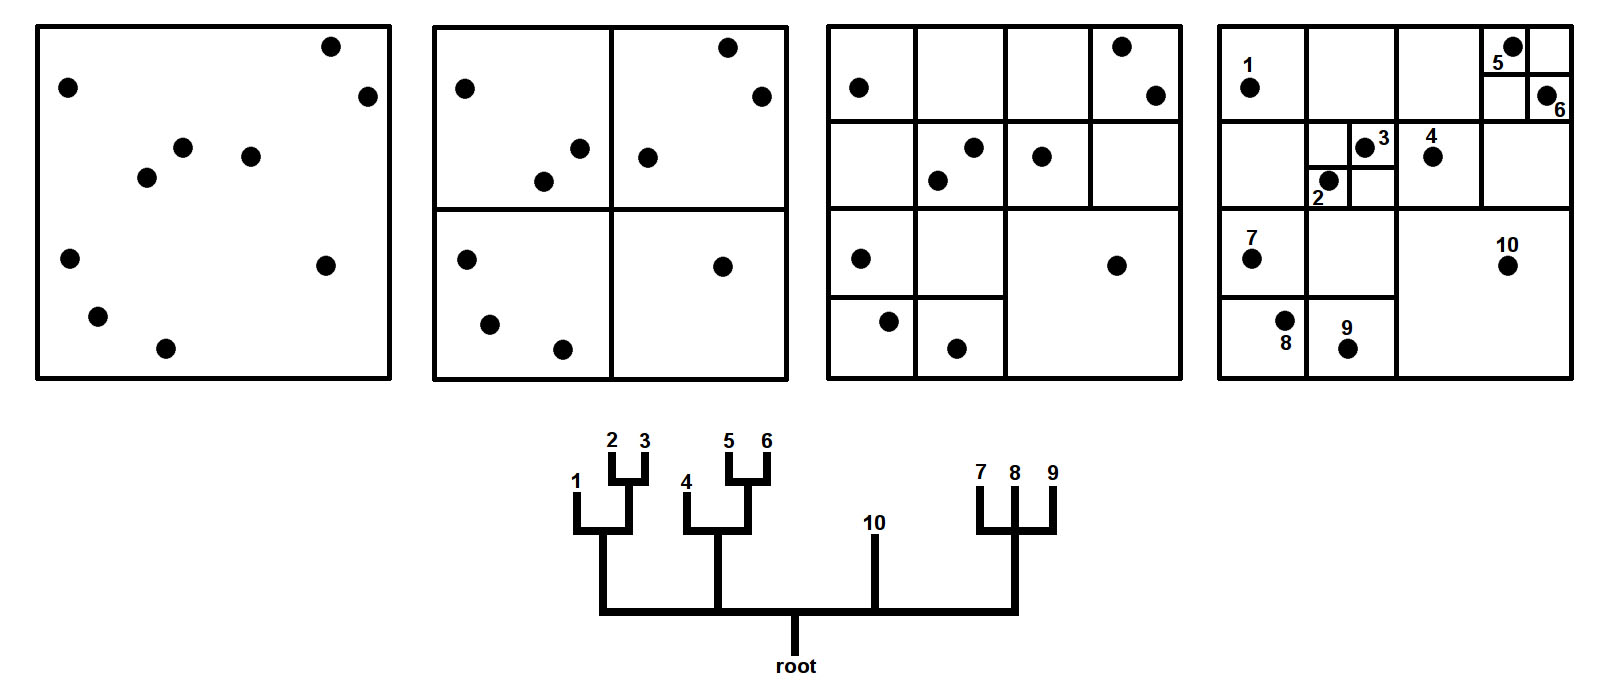
\includegraphics[width=.95 \textwidth]{Pictures/9/treecode.jpg}
    \caption{Funzionamento di un tree code in due dimensioni. L'albero generato alla fine del processo ha 3 livelli. Per esempio, per calcolare la forza che agisce sulla particella 8 si calcola la distanza dal baricentro dei quadratoni tracciati al secondo step. Quello in alto a destra può essere considerato sufficientemente lontano: le particelle 4, 5, 6 vengono viste come un'unica particellona. Il quadrato in basso a destra viene preso così com'è perché contiene già solo una particella. }\label{fig9:treecode}
\end{figure}
\end{example}  

\noindent Test possibili:
\begin{itemize}
    \item Conservazione di massa (particelle), energia (facile su intervalli temporali piccoli)
    \item Conservazione del momento (se una particella esce da un bordo, deve entrare dall'altro)
\end{itemize}

\noindent Condizioni iniziali:
\begin{itemize}
    \item Modello cosmologico con perturbazioni gaussiane
    \item Realizzazioni random dello spettro di potenza 
    \item Appossimazione di Zeldovich (particelle + piccola perturbazione) $\to$ $n,A,T(k)$
    \item Ora può avere inizio la simulazione non lineare con uno dei metodi descritti
\end{itemize}

Metà della cosmologià è stata fatta col codice GADGET perché il signor Springel lo ha reso pubblico, nella versione attuale è un albero combinato con PM. Oggi le simulazioni più grandi hanno più di $10^{10}$ particelle, raggiunte per la prima volta dalla simulazione Millennium (box di $500$ Mpc/h). Questa ha richiesto l'equivalente di 343`000 ore di calcolo (parallelizzato in circa $1$ mese) e ha prodotto 27TB di dati. Si può osservare la formazione della Cosmic Web e l'allargamento dei vuoti. Da queste simulazioni possono essere aggiunti a mano i barioni, se ne studia l'evoluzione e si confronta con i risultati osservativi (modelli semianalitici). Infatti generalmente viene incluso soltanto il contributo della dark matter.

Inoltre, si può studiare il collasso ellissoidale (Sheth e Tormen) e vedere come questo riproduca i dati simulati meglio di quello di Press–Schechter.

Infine si può studiare l'evoluzione del clustering (prima piani e poi filamenti) al variare del tempo. In questo modo si possono avere relazioni anche non lineari che mostrano l'evoluzione in redshift. Un modo intelligente è quello di seguire le strutture formate con griglie più definite, mantenendo comunque memoria dell'environment. In queste simulazioni \textit{zoomed} si inetteno modi di piccola frequenza nelle regioni interessate dalla formazione di strutture che possono sempre essere ricondotti alla \textit{parent simulation} (si può aumentare la risoluzione fino a 3 dex). Sui singoli ammassi oggi si può arrivare anche a un miliardo di particelle.

Una delle predizioni che nasce dalle simulazioni numeriche è l'esistenza di profili di distribuzione della densità di dark matter autosimilari, ossia i profili NFW ($r{-1}$ a piccoli raggi, $r^{-3}$ a grandi raggi). 

\subsection{Gastrofisica}
In base alle relazioni di scala ottenute, un ammasso globulare dovrebbe essere una fotocopia di un ammasso di galassie. I barioni sono pochi, ma creano un gran casino e sono complessi da trattare. Tuttavia buona parte delle osservazioni si basa su di loro, quindi le simulazioni devono essere migliorate. Questo è difficile quando le singole particelle hanno massa di $10^5 M_\odot$ a causa della risoluzione limitata della simulazione.

Generalmente le leggi idrodinamiche possono essere riscritte sotto forma di equazioni differenziali di conservazione del flusso. In idrodinamica di sono due approcci molto diversi: euleriani e lagrangiani. 

I primi sono basati sull'utilizzo di griglie, mediando le quantità fisiche senza seguire il moto delle particelle. La griglia eventualmente può essere resa adattiva. Il vantaggio è che i gradienti (shock) possono essere descritti bene, però allo stesso tempo si stanno ignorando tutti i fenomeni che avvengono sotto-griglia. Il metodo più semplice per risolvere queste equazioni differenziali è quello di Eulero, più furbo è quello PPM (Picewise Parabolic Method, la regione di influenza su una cella non è legata al valore medio ma ad uno smussamento parabolico delle celle adiacenti). 

Gli approcci lagrangiani si basano sul seguire le particelle e le loro interazioni. Non si utilizza una griglia. Se le particelle clusterano si ha alta risuluzione, al contrario non si ha sufficiente informazione per calcolare la densità dei vuoti. Nascono problemi di risoluzione delle equazioni che vanno risolti introducendo una viscosità artificiale. Uno dei metodi migliori è l'SPH (Smoothed Particle Hydrodynamics): ogni particella si porta dietro le quantità medie locali. Per calcolare le quantità totali non è sempre necessario sommare su tutte le particelle: molte forze che agiscono sono a corto raggio (in gen $\sim 30$ particelle). Inoltre molte equazioni possono essere riscritte col formalismo dell'SPH per il quale vale: $\left\langle \rho (r)\right\rangle =\int\rho(r-r')W\d{V}\to \left\langle \rho_i\right\rangle= \sum \frac{m_j}{\rho_j}\rho_j W$, ossia gli operatori sono lineari: derivate e integrali diventano somme.  

Nel 1999 è stato fatto un esperimento per confrontare i due metodi (Santa Barbara Comparison) con codici scritti da gruppi diversi. Trattando il gas sembrava che nulla tornasse ed essendo evoluzioni non lineari non si capiva chi potesse avere ragione. I codici lagrangiani sono più naturali per le simulazioni n-body, mentre quelli euleriani per la gastrofisica. In realtà si è capito che è tutto dipendente dalla risoluzione del codice e oggi i risultati sono compatibili. I metodi euleriani e lagrangiani hanno ripettivamente: alta/bassa risoluzione in massa e bassa/alta risoluzione spaziale.

Alcuni risultati ottenibili dai modelli riguardano: profili di densità dei cluster (non NFW col gas perchè collisionale), profili di temperatura dei cluster (non isotermi), distribuzione di entropia del gas (deviazione dall'autosimilarità: heating non gravitazionale e cooling), deviazioni dalle relazioni di scala per oggetti piccoli. 

I codici devono soddisfare le osservazioni: bubbles nell'IC, turbolenza, misure di rotazione nei lobi delle radiogalassie (campi magnetici), feedback degli AGN (arricchimento dell'ICM, conduzione termica). 

In conclusione, la gravità è sotto controllo (a parte qualche problemino nelle regioni più compatte), i metodi diversi convergono, ma le simulazioni sono ancora lontane dall'essere realistiche. 

